% TODO: Extract to settings.tex

% Variables and other equation stuff
\newcommand{\Q}{\bm{Q}}
\newcommand{\gradQ}{\gradient{\Q}}
\newcommand{\Qrho}{\rho}
\newcommand{\Qj}{\rho \bm{v}}
\newcommand{\Qv}{\bm{v}}
\newcommand{\QE}{\rho E}
\newcommand{\QZZ}{Z} % TODO: Name?
\newcommand{\QZ}{\rho \QZZ}
\newcommand{\potT}{\theta}
\newcommand{\backgroundPotT}{\overline{\theta}}
\newcommand{\pertubationPotT}{\theta'}
\newcommand{\stressT}{\bm{\sigma}}
\newcommand{\pressure}{p}
\newcommand{\maxConvEigen}[1][]{
  \vert%
  \lambda_c^{\text{max}}
  \notblank{#1}{\left(#1\right)}{}
  \vert%
}
\newcommand{\maxViscEigen}[1][]{
  \vert%
  \lambda_v^{\text{max}}
  \notblank{#1}{\left(#1\right)}{}
  \vert%
}
\newcommand{\Riemann}{\operatorname{Riemann}}

% Stuff for numerics
\newcommand{\domain}{\Omega}
\newcommand{\broken}{\domain}
\newcommand{\cell}[1][]{C_{#1}}
\newcommand{\boundary}{\partial \domain}
\NewDocumentCommand{\sbasis}{ O{} O{} }{\phi^{#1}_{#2}}
\NewDocumentCommand{\stbasis}{ O{} O{} }{ \Theta^{#1}_{#2}}
\NewDocumentCommand{\sbasisRef}{ O{} O{} }{\hat{\sbasis[#1][#2]}}
\NewDocumentCommand{\stbasisRef}{ O{} O{} }{\hat{\stbasis[#1][#2]}}
%\newcommand{\stestfunction}[1]{\sbasis[#1]}
\NewDocumentCommand{\stestfunction}{ O{} O{} }{\sbasis[#1][#2]}
\NewDocumentCommand{\sttestfunction}{ O{} O{} }{\stbasis[#1][#2]}
\newcommand{\normal}{\bm{n}}
\newcommand{\dsol}[1][h]{\bm{u}_{#1}}
\newcommand{\stpredictor}[1][h]{\bm{q}_{#1}}

% Equation parts
\newcommand{\flux}{F}
\newcommand{\viscFlux}{\flux^{v}}
\newcommand{\hyperFlux}{\flux^{h}}
%\newcommand{\source}{\bm{S}}
\newcommand{\source}[1][]{
  \notblank{#1}{
S_{#1}
}{
\bm{S}
}
}

% Integrals
\newcommand{\intdt}[1]{\int_{t^n}^{t^{n+1}} #1 \dd{t}}
\newcommand{\intdcell}[1]{\int_{\cell} #1 \dd{\bm{x}}}
\newcommand{\intdrefcell}[1]{\int_{\cell} #1 \dd{\hat{\bm{x}}}}
\newcommand{\intdcellb}[1]{\int_{\partial{} \cell} #1 \dd{S}} % TODO: define boundary of cell
\newcommand{\intdrefcellb}[1]{\int_{\partial{} \cell} #1 \hat{\dd{S}}} % TODO: define boundary of cell

% Yet to be sorted
\newcommand{\quadWeight}[1][i]{w_{#1}}

\chapter{An ADER-DG scheme for the Navier-Stokes Equations}\label{chap:methods}
This chapter describes the numerical and physical background that is needed to simulate reacting fluids with good accuracy.
We start with a description 
We start with a description of the arbitrary high order derivatives (\ader) discontinuous Galerkin (\dg) method with a focus on equations that contain both advective and diffusive terms.
We then seque into a short description of the \muscl\ scheme, a second order finite volume scheme.

We conclude this chapter by a description of adaptive mesh refinement (\amr) and finite volume limiting, which combines both numerical methods to achieve a stable, high-order method.

\section{Reactive Compressible Navier Stokes Equations}\label{sec:navier-stokes}
\newcommand{\diffCoeff}{\varepsilon}
\newcommand{\hyperFluxDef}{
  \begin{pmatrix}
    \Qj \\
    \Qv  \otimes \Qj + \bm{I} \pressure  \\
    \Qv \cdot (\bm{I} \QE + \bm{I} \pressure) \\
    \Qj \QZZ
  \end{pmatrix}
}

\newcommand{\viscFluxDef}{
  \begin{pmatrix}
     -\diffCoeff \gradient{\Qrho}\\
     \stressT (\Q, \gradQ)  \\
     \Qv \cdot \stressT (\Q, \gradQ) - \kappa \gradient{T}\\
     -\diffCoeff \gradient{\QZ}
   \end{pmatrix}
}

Fluid motion can be described by the compressible Navier Stokes equations.
We follow the description in~\cite{dumbser2010arbitrary} for the Navier Stokes part.
The coupling with the advection-diffusion-reaction equation follows~\cite{hidalgo2011ader} which describes this equation set for the one-dimensional case.
In the following, we will denote the spatial coordinates as $\bm{x} = \left( x,z \right)$ and $\bm{x} = \left( x,y,z \right)$ for the two and three-dimensional case respectively.
The variable $t$ corresponds to the currenty (physical) time.
We solve the \pde\ in the conversative form \pcref{eq:conservation-law-gradient}\todo{Dont reference to following chapter!}
\begin{equation}
 \label{eq:equation-set} 
 \begin{array}{l}
 \text{mass cons.} \\
 \text{momentum cons.} \\
 \text{energy cons.} \\
 \text{cont.\ gas} 
\end{array}
:
\quad
  \pdv{}{t}
  \underbrace{
  \begin{pmatrix}
    \Qrho\\
    \Qj\\
    \QE\\
    \QZ
    \end{pmatrix}}_{\Q}
  +
  \divergence{
  \underbrace{
  \left(
   \underbrace{\hyperFluxDef}_{\hyperFlux(\Q)}
+
\underbrace{\viscFluxDef}_{\viscFlux(\Q, \gradQ)}
  \right)}_{\flux(\Q, \gradQ)}}
 =
  \underbrace{
  \begin{pmatrix}
    \source[\Qrho\phantom{\Qrho}]\\
    \source[\Qj]\\
    \source[\QE]\\
    \source[\QZ]
    \end{pmatrix}}_{\source(\Q, \bm{x}, t)}
\end{equation}
which describes the time evolution of variables $\Q$ with respect to a flux $\flux(\Q, \gradQ)$ and a source $\source(\Q)$.
The vector of conserved quantities is given by
\begin{equation}
  \label{eq:conserved-variables}
 \Q = \left( \Qrho, \Qj, \QE, \QZ \right),
\end{equation}
where $\Qrho$ is the density, $\Qj$ is the two or three-dimensional momentum, $\QE$ the energy density and $\QZ$ is the mass fraction of the chemical reactant.
The chemical reactant in our case is unburnt gas.

The rows of the equation are the conservation of mass, the conservation of momentum, the conservation of energy and the continuity of the reactant.
We split the flux into a hyperbolic $\hyperFlux(\Q)$ and a viscous part$\viscFlux(\gradQ)$

\begin{equation}
  \label{eq:flux}
  \flux(\Q, \gradQ) = \hyperFlux(\Q) + \viscFlux(\Q, \gradQ).
\end{equation}
The hyperbolic flux is given by
\begin{equation}
  \label{eq:hyper-flux}
  \hyperFlux(\Q) = \hyperFluxDef,
\end{equation}
which are the Euler equations coupled with an advection equation.
In this equation $\bm{a} \otimes \bm{b} = \bm{a} \bm{b}^\intercal$ is the Kronecker or outer product of two vectors $\bm{a}$ and $\bm{b}$.
The pressure $\pressure$ is given by the caloric equation of state of an ideal reacting gas\todo{Geopot height correct?}
\begin{equation}
  \label{eq:eos}
  \pressure = (\gamma - 1) \left(\QE - \frac{1}{2} \left(\Qv \cdot \Qj \right)  - q_0 \QZ - gz \right).
\end{equation}
The term $q_0 \QZ$ is the chemical energy with the heat release $q_0$, the term $gz$ is the geopotential height.
The pressure is related to the temperature $T$ by the thermic ideal gas law
\begin{equation}
  \label{eq:temperature}
 \frac{\pressure}{\Qrho} = RT,
\end{equation}
where $R$ is the specific gas constant of a fluid.

The viscous flux is
\begin{equation}
  \label{eq:visc-flux}
  \viscFlux(\Q, \gradQ) = \viscFluxDef.
\end{equation}
where $\stressT$ and $(\kappa \nabla T)$ denote the stress tensor and heat flux respectively.
The viscous effects of the fluid are modeled by the stress tensor
\begin{equation}
  \label{eq:stress-tensor}
  \stressT(Q, \nabla Q) =
  \mu
  \left(
  \left(\nicefrac{2}{3} \divergence{\Qv} \right) -
  \left( \gradient{\Qv} + \gradient{\Qv}^\intercal \right)
  \right).
\end{equation}

We further introduce the ratio of specific heats $\gamma$ and the heat fraction for constant volume $c_v$ and constant volume $c_r$.
These constants are all fluid dependent and relate to each other and the gas constant by
\begin{align}
  \label{eq:fluid-constants}
  \begin{split}
  c_v &= \frac{1}{\gamma - 1} R \\
  c_p &= \frac{\gamma}{\gamma - 1} R\\
  R &= c_p - c_v\\
  \gamma &= \frac{c_p}{c_v}.
  \end{split}
\end{align}
\todo{Cite sth for this!}
We can then compute the heat conduction coefficient
\begin{equation}
  \label{eq:heat-conduction-coeff}
  \kappa = \frac{\mu \gamma}{\Pr} \frac{1}{\gamma - 1} R = \frac{\mu \gamma}{\Pr} c_v,
\end{equation}
where the Prandtl number $\Pr$ depends on the fluid.
% Sutherland's viscosity law:
% \begin{equation}
%   \label{eq:sutherland}
%  \mu(T)  = \mu_0 {\left(\frac{T}{T_0}  \right)}^{\beta} \frac{T_0 + C}{T + C}
% \end{equation}
% with \(\beta = 1.5\), \(C = \text{const.}\), reference temperature $T_0$ and reference viscosity $\mu_=$.
% Equal to
% \begin{align}
%   \lambda &= \frac{\mu_0 (T_0 + C)}{T_0^\beta} \\
%   \mu(T) &= \lambda \frac{T^\beta}{T + C},
% \end{align}
% where $\lambda$ is constant for a given fluid.

The maximal absolute eigenvalues for convective and viscous part in direction of a normal vector $\normal$ are
\begin{align}
  \begin{split}
    \maxConvEigen &= \left( \partial \bm{F}/\partial \bm{Q}\right) \cdot \normal = \vert \Qv_{\normal} \vert + c,\\
    \maxViscEigen &= \left( \partial \bm{F}/\partial \left( \nabla \bm{Q} \cdot \normal \right)\right) \cdot \normal =
    \max \left( \frac{4}{3} \frac{\mu}{\Qrho},
                        \frac{\gamma \mu}{\Pr \Qrho},
                        \diffCoeff \right)
  \end{split}
\end{align}
with velocity in direction of the normal $\Qv_{\normal}$ and speed of sound $c = \sqrt{\gamma R T }$.

We also support two different kind of (optional) source terms.
\todo{Either include gravity in pressure or add source term for energy.}
The first source term is gravity, given by
\begin{equation}\label{eq:source-gravity}
  \source[\Qj] = - g \bm{k} \cdot \Qj,
\end{equation}
where $g = 9.81$ and $\bm{k}$ is a unit vector pointing in $z$-direction.

\newcommand{\backgroundPressure}{\overline{\pressure}}
\newcommand{\backgroundRho}{\overline{\Qrho}}
Some of our scenarios can be described as a pertubation of a background state that is in hydrostatic balance
\begin{equation}
  \label{eq:hydrostatic-balance}
  \pdv{}{z} \backgroundPressure{\left (z \right )} = -g \backgroundRho(z),
\end{equation}
where $\backgroundPressure$ and $\backgroundRho$ is the background pressure and density.
We now focus on the following part of the momentum equation (neglecting viscous effects) of \cref{eq:equation-set}
\begin{equation}
  \label{eq:momentum-equation}
  \pdv{\Qj}{t}+ \divergence{
    \Qv \cdot \left( \bm{I} \QE + \bm{I} \pressure \right)
  }
  =
  -g \bm{k} \cdot \Qrho
\end{equation}.
The background state \cref{eq:hydrostatic-balance} leads to large values and can diminish other parts of the flux due to numerical instabilities~\cite{muller2010adaptive}.
We can now split the pressure as $\pressure = \backgroundPressure(z) + \pressure' (\bm{x}, t)$ and the density as $\Qrho = \backgroundRho(z) + \Qrho'(\bm{x}, t)$.
Inserting this splitting, the definition of divergence into \cref{eq:momentum-equation} allows us to apply \cref{eq:hydrostatic-balance}.
Furthermore, the background states have zero derivatives in all directions but in $z$.
We arrive at 
\begin{equation}
  \label{eq:momentum-equation}
  \pdv{\Qj}{t}+ \divergence \left(
    \Qv \cdot \left( \bm{I} \QE + \bm{I} \pressure' \right)
   \right)
  =
  -g \bm{k} \Qrho'.
\end{equation}.
We thus cancel parts of the flux with parts of the source term.
Note that the time derivative of the background density also vanishes.
We do not use this to simplify the implementation of the gradient computation.
This form of the equation is similar to equation set 3 of~\cite{giraldo2008study} but without splitting the energy.

\newcommand{\reactionTimescale}{\tau}
\newcommand{\reactionTemperature}{T_{\text{ign}}}
The chemical reactive source term is
\begin{equation}\label{eq:source-reaction}
  \source[\QZ] = - K(T) \QZ.
\end{equation}
We use the very simple reaction model
\begin{equation}\label{eq:reaction-model}
\begin{cases}
  - \frac{1}{\reactionTimescale} & T > \reactionTemperature\\
  0 & \text{otherwise}
\end{cases}  
\end{equation}
where $\reactionTimescale$ is the timescale of the reaction and $\reactionTemperature$ is the activation temperature.

\subsection{Boundary conditions}
To close the system we need to impose boundary conditions.

\sidetitle{Cauchy}
For some scenarios we use Cauchy boundary conditions.
In most cases, we would like to impose periodic boundary conditions, due to the inner workings of \exahype{} this is not possible.
Instead we use the analytical solution of our problems at the boundary, imposing both value and gradients of the conservative variables.
Note that this leads to an error when our problem does not posses an exact analytical solution.
This is the case for test cases that are analytical solutions to the incompressible Navier Stokes equations but do not satisfy the compressible equation set.

As a physical boundary condition we limit ourselves to wall boundary condition

\sidetitle{No-Slip}
A standard wall boundary condition for viscous fluid is the no-slip condition, where we assume that the fluid has a velocity of zero near the wall.
\todo{Check if this is the correct physical description!}
We enfore this by setting
\begin{align}
  \label{eq:no-slip}
  \begin{split}
  \Qrho^o &= \Qrho^i, \\
  \Qj^o &= -\Qj^i, \\
  \QE^0 &= \QE^i,\\
  {(\nabla Q)}^o &= {(\nabla Q)}^i,
  \end{split}
\end{align}
where a superscript of $o$ and $i$ denotes the values outside and inside of the boundary respectively.

\sidetitle{Free-Slip}
Similarly to the no-slip condition, we define the free-slip condition
\begin{equation}
  \label{eq:free-slip}
  \Qj^o_d = \begin{cases}
    -\Qj^i_d & d = \text{normal} \\
    \Qj^i_d & \text{otherwise}
    \end{cases}
\end{equation}
where only the velocity in normal direction is zero after the Riemann solver.
The other variables are extrapolated in the same manner as in \cref{eq:no-slip}.

We manually set the energy component of the numerical flux to zero for both no- and free-slip conditions.
\section{The ADER-DG Method}\label{sec:ader-dg}
We describe the arbitrary derivative discontinous Galerkin (\aderdg) method in this chapter.
Our description of the main method follows~\cite{dumbser2008unified,dumbser2010arbitrary,dumbser2018efficient}, our notation follows primarily~\cite{dumbser2018efficient}.
We discuss the approximation of systems of partial differential equations (\pde) of the form
\begin{equation}
  \label{eq:conservation-law-gradient}
 \frac{\partial}{\partial_t}  \Q + \div \flux(\Q, \gradQ) = \source(\bm{x}, t, \Q),
\end{equation}
which in contrast to hyperbolic conservation laws of the form
\begin{equation}
  \label{eq:conservation-law}
 \frac{\partial}{\partial_t}  \Q + \div \flux(\Q) = \source(\bm{x}, t, \Q)
\end{equation}
contain the gradient $\gradQ$ of the so called vector of conservative variables $\Q$~\cite{dumbser2010arbitrary}.
There are therefore not hyperbolic but rather parabolic or elliptic.

We discuss the solution of a hyperbolic conservation law \cref{eq:conservation-law} with domain $\domain$ and boundary $\boundary$.
Let $\domain$ and $\boundary$ denote our two- or three-dimensional computational domain and its boundary.
In our implementation of the discontinous Galerkin (\dg) framework, we approximate this solution in the space
\begin{equation}
  \label{eq:dg-space}
  \broken = \bigcup_i \cell
\end{equation}
of disjoint quadrilateral cells $\cell$.
Note that we do not distinguish between the broken approximation space and the domain, the use should be clear given its surrounding context.
In the following we make use of the Einstein summation convention where summation over repeated indexes is implied.

% Inside each cell $\cell$ we represent the solution in terms of the basis function 
% \begin{equation}
%   \label{eq:cell-approx}
%   u(\bm{x}, t^n)_{|\cell[i]} = \hat{u}^n_{i,l} \sbasis{l}(\bm{x}),
% \end{equation}
% where $l$ is a multi-index, containing one index per spatial dimension.
% \todo{dofs $\hat{u}$, local solution, etc.}
% For example, $(l = (l_1, l_2))$ for the two dimensional case.
% This polynomial is interpolating, i.e.\ \ldots\todo{interpolating?}.
% This choice of basis (called \textit{nodal} basis) allows us to easily compute integrals over cells using Gaussian quadrature.
% In detail, we use a the Lagrange interpolation polynomials.

We now describe the derivation of the \textsc{ader-dg} method.
This scheme is a predictor-corrector method.
We first compute a local time evolution of each cell in a predictor step and then add the influence of the neighbors in the corrector step.
$\ldots$

% \begin{algorithm}[H]
%   \begin{algorithmic}
%     \Let{$\stpredictor$}{Initial guess}
%     \Let{$F_h$}{$\flux(\Q, \gradQ)$}
%     \Let{$\stpredictor$}{Solve \cref{eq:space-time-predictor} using $F_h, \Q, \gradQ$}
%     \Let{$\left( \hat{F_h}, \hat{\Q}, \hat{\gradQ}, \hat{\stpredictor} \right)$}
%         {Extrapolate to boundary using \cref{eq:boundary-extrapolation}}
%     \Let{update}{Use \cref{eq:corrector} with boundary extrapolated values (fluxes of neighbors)}
%   \end{algorithmic}
%   \caption{The \textsc{ader-dg} algorithm for one cell.}
% \end{algorithm}

\sidetitle{Reference Cell}
\newcommand{\mapping}{\mathcal{M}}
\newcommand{\volume}{V}
For reasons of computational efficiency, we describe the scheme in terms of a reference cell.
We use the quad cell $\cell = [0, 1]^D$\todo{check if $[0,1]$ detontes correct interval}.
The mapping, which takes a point on the reference cell with coordinates $\hat{\bm{x}}$ and returns a point $\bm{x}$ on a cell with center and widths $(\Delta x, \Delta y, \Delta z)$, is given by
\begin{equation}\label{eq:space-mapping}
  \hat{x} = \mapping (\bm{x}) =
  \operatorname{cell-center}(\cell) +
\begin{pmatrix}
\Delta x && \\
&\Delta y & \\
&&\Delta z&
\end{pmatrix}
 % \operatorname{diag}(\Delta x, \Delta y, \Delta z)
  \begin{pmatrix}
    x - 0.5\\
    y - 0.5\\
    z - 0.5
  \end{pmatrix}.
\end{equation}

We also define the inverse mapping $\mapping^{-1}$.
This can be used to define a function $f(\bm{x})$ acting on a point $\bm{x}$ of a regular cell in term of a function $\hat{f}(\bm{x})$ that acts on a point of the reference cell by considering
\begin{equation}
  \label{eq:function-ref-cell}
  f(\bm{x}) = f\left( \mapping^{-1}(\bm{x}) \right) = \hat{f}(\hat{\bm{x}}).
\end{equation}

Similar to this, we define a mapping that maps a point in time to the reference time $\in (0,1)$
\todo{Fix this/remove}
\newcommand{\timeMapping}{\mathcal{T}}
\begin{equation}
  \label{eq:time-mapping}
  \hat{t} = \timeMapping(t) = t_0 + (\Delta t) t,
\end{equation}
where $\Delta t$ is timestep of a cell and $t_0$ is the beginning of its time interval.

The Jacobian determinant of $\mapping$ is simply the volume $V$ of the cell
\begin{equation}
  \label{eq:determinant-mapping}
  \volume = \operatorname{det}(\operatorname{Jacobian}\mapping) = \Delta x \, \Delta y \,\Delta z,
\end{equation}
the Jacobian determinant of $\timeMapping$ is $\Delta t$.
This is useful for evaluating derivatives by the chain rule and, similarly, integrals by substitution.
For example, we can evaluate a volume integral by
\begin{equation}
  \label{eq:integration-by-substitution}
  \intdcell{
f(\bm{x})
  }
  =
\volume \intdrefcell{
    \hat{f}(\hat{\bm{x}})
  }
\end{equation}
\sidetitle{Basis Functions}
\newcommand{\lagrangeRef}[1][i]{\hat{L}_{#1}}
\newcommand{\lagrange}[1][i]{L_{#1}}
The next step is the definition of basis functions for the reference cell.
We use Langrange polynomials that are defined in the one-dimensional case by
\begin{equation}
  \label{eq:lagrange-basis}
  \lagrangeRef(x) = \prod_{i \neq j}^N \frac{x - x_j}{x_i - x_j}.
\end{equation}
We can then represent functions as a sum over the support points $x_j$
\begin{equation}
  \label{eq:langrange-expansion-1d}
  f(x) = \sum_{i = 0}^N f(x_i) \lagrangeRef[i](x) = f(x_i) \lagrangeRef[i](x),
\end{equation}
where we used the Einstein summation convention where summation over repeated indices is implied.
The support points $x_i$ are chosen such that they coincide with the nodes of the Gauss-Legendre quadrature which we can use to evaluate integrals
\begin{equation}
  \label{eq:quadrature-1d}
  \int_0^1 f(x) \dd{x} = \sum_n^N \quadWeight[n] f(x_n),
\end{equation}
where $x_n$ is a quadrature point with weight $\quadWeight[n]$.
The basis functions are similarly defined in $d$ dimensions by considering nodes that are the tensor-products of $d$ one-dimensional Gauss-Legendre quadrature.
To simplify notation, we order the polynomials by a linearised index, a $d$-dimensional function is then approximated by
\begin{equation}
  \label{eq:lagrange-expansion}
  f(\bm{x}) = \sum_{i = 0}^{N^d} f(\bm{x}_i) \lagrangeRef[i](\bm{x}) = f(\bm{x}_i) \lagrangeRef[i](\bm{x}).
\end{equation}
Similarly to the one-dimensional case, we can evaluate integrals by
\begin{align}
  \label{eq:quadrature}
  \underbrace{\int_0^1 \cdots \int_0^1}_{D \text{ times}} f(\bm{x}) \dd{\bm{x}} &= \sum_n^{(N+1)^D - 1} \quadWeight[n] f(\bm{x}_n) \\
  \intertext{with}
  \quadWeight[n] &= \prod_{i}^{d} \quadWeight[i].
\end{align}
\todo{Fix notation, especially multi-dimensional integral.}
\todo{Check number of total polynomials.}
% TODO: Quadrature

Two important properties of this family of polynomials are
  \begin{alignat}{10}
    \label{eq:basis-interpolating}
&& \text{Interpolating:} \qquad & \lagrangeRef[i] (x_j) &= \delta_{ij}\\
\label{eq:basis-orthogonality}
&& \text{Orthogonality:} \qquad &
\int_0^1 \cdots \int_0^1 \lagrangeRef[j](\hat{\bm(x)} \lagrangeRef[j]{\hat{\bm{x}}}) \dd{\hat{\bm{x}}}  &= \quadWeight[i] \delta_{ij}
    \end{alignat}

We will later need basis functions over a space-cell 
\begin{align}\label{eq:space-basis}
  \begin{split}
  \sbasisRef(\hat{\bm{x}}) &= \sum_i^{(N+1)^D - 1} \lagrange[i] (x_i)\\
  \sbasis(\bm{x}) &= \sbasisRef \left( \mapping(\bm{x}) \right)
  \end{split}
\end{align}
where $\sbasisRef$ denotes the basis function on the reference cell.
Similarly, we define a basis for a space-time element defined by $(0, 1)^D \times (t^n, t^{n+1})$
\begin{align}\label{eq:space-time-basis}
  \begin{split}
  \stbasisRef(\hat{\bm{x}}, \hat{t}) &= \sum_j^{N} \sum_i^{(N+1)^D - 1} \lagrange[j](x_j) \lagrange[i] (x_i)\\
  \stbasis (\bm{x}, t) &= \stbasisRef \left( \mapping(\bm{x}), \timeMapping(t) \right)
  \end{split}
\end{align}

\sidetitle{Predictor}
To derive the predictor, we take an approximation of our solution in a nodal basis that is defined both in space and time
\begin{equation}
  \label{eq:cell-approx-space-time}
  q(\bm{x}, t^n)_{|\cell[i]} = \hat{u}^n_{i,l} \stbasis[][l](\bm{x}, t).
\end{equation}
Furthermore we assume that all quantities are given in this represantation.
We now multiply the conservation law by a test function (of the same function space as the basis) and arrive at the weak formulation
\begin{equation}\label{eq:weak-pde-space-time}
\intdt{\intdcell{
    \sttestfunction{k}(\bm{x}, t)
    \pdv{\stpredictor}{t}
}}
+
\intdt{\intdcell{
    \sttestfunction{k}(\bm{x}, t)
    \left(
      \divergence{\flux(\stpredictor, \gradient{\stpredictor})}
    \right)
}}
=
\intdt{\intdcell{
  \sttestfunction{k} \source(\stpredictor)
}}.
\end{equation}
We integrate the first term by parts in time and the flux divergence in space.
Here we do not use the Riemann solver for the flux boundary term but rather use the discrete solution at time $t$.
This corresponds to upwinding in time~\cite{dumbser2008unified}.
Note that this neglects the interaction with neighbouring cells.
We account for this in the corrector step.
\begin{align}\label{eq:space-time-predictor}
\begin{split}
\intdcell{
  \sttestfunction{k} (\bm{x}, t^{n+1}) \stpredictor(\bm{x}, t^{n+1})
}
&-
\intdt{\intdcell{
    \pdv{}{t} \sttestfunction{k}(\bm{x}, t) \stpredictor(\bm{x}, t)
}}
= \\
\intdcell{
  \sttestfunction{k}(\bm{x},t^n) \dsol(\bm{x}, t^n)
}
&+
\intdt{\intdcell{
    \sttestfunction{k}(\bm{x},t) \divergence{\flux(\stpredictor, \gradient{\stpredictor})}
}}
+
\intdt{\intdcell{
    \sttestfunction{k}(\bm{x}, t) \source(\stpredictor)
}}
\end{split}
\end{align}
Inserting \cref{eq:cell-approx-space-time} results in a local systems of equations that can be by a fixed point iteration scheme.
\todo{Inital guess correct? Maybe cite sth?}
As initial value for the space-time-predictor we use the solution of the timestep before.
\todo{Collect into matrices and show scheme?}
To show the computational efficiency of our scheme, we follow the approach of~\cite{dumbser2008unified} and collect our integrals into matrices\todo{Source is Dominics \aderdg-document.}.

\newcommand{\pleft}{\bm{L}}
\newcommand{\prightsol}{\bm{r}}
\newcommand{\prightpred}{\bm{w}}
\begin{align}
  \label{eq:predictor-matrices}
  \pleft^{\cell}_{(n v l), (n' v' l')} &=
\intdcell{
  \sttestfunction[\cell][v,l,n](1) \stbasis[\cell][v,l', n']
}
-
\intdt{\intdcell{
  \left( \pdv{}{t} \sttestfunction[\cell][v,l,n] (t) \right) \stbasis[\cell][v,l',n']
}}                             
\\
\prightsol^{\cell}_{v, l,n} &=
\intdcell{
  \sttestfunction[\cell][v,l,n] (0) \sbasis[\cell][v,n'] \dsol[v,n']^{\cell}
}
+
\intdt{\intdcell{
  \sttestfunction[\cell][v,l,n] \stbasis[\cell][v,l',n'](t) S_{v,l',n'}(\stpredictor[]^{\cell, i})
}}                             
  \\
\prightpred^{\cell}_{v,l,n} &= 
F^{k}_{v,l',n'}
\intdt{\intdcell{
  \left( \gradient{\sttestfunction[\cell][v,l,n]} \right) \stbasis[\cell][v,l',n'](t) S_{v,l',n'}(\stpredictor[]^{\cell, i})
}}
\end{align}
Using these matrices, we can solve for the space-time-predictor with the iterative scheme
\begin{align}
  \label{eq:predictor-iterative}
  \pleft \stpredictor[]^{\cell, i+1} &= \prightsol (\dsol) - \prightpred(\stpredictor[]^{\cell, i}) \\
 \stpredictor[]^{\cell, i+1} &= \pleft^{-1} \left( \prightsol (\dsol) - \prightpred(\stpredictor[]^{\cell, i}) \right).
\end{align}
For details and proof of convergence for the linear case, see~\cite{dumbser2008unified}.

\sidetitle{Preparing for corrector}
We then prepare the space-time-predictor for use in the corrector step.
Due to the linearity of the Riemann solver, we can exchange time and space integration and thus only need to consider the Riemann problem for time-averaged quantities.
% We can compute this for the space-time-predictor by
% \begin{align}
%   \ldots = \ldots,
% \end{align}
% the procedure is similar for all other quantities (Q, gradQ, fluxes).
We then extrapolate all quantities to the boundary.
This is needed for the Riemann solver and for the reconstruction of boundary values.
We accomplish this by evaluating the function at the degrees of freedom on the boundary.
Thanks to the interpolating property of the nodal basis~\pcref{eq:basis-interpolating}, this reduces to a change of basis which can be precomputed on the reference element.
We compute time-averaged and boundary extrapolated versions of the space-time-predictor, the degrees of freedom and their gradient, and the fluxes. 

\sidetitle{Corrector}
The final step of the \aderdg{}-scheme is the corrector.
For this step, we write the approximation of a function $q$ in a cell as
\begin{equation}
  \label{eq:cell-approx-space}
  q(\bm{x})_{|\cell[i]} = \hat{u}^n_{i,l} \sbasis{l}(\bm{x}),
\end{equation}
where the basis, unlike in \cref{eq:cell-approx-time}, does not depend on the time.
We then multiply the system \cref{eq:conservation-law-gradient} by a test function $\stestfunction{i}$ and integrate over the space-time volume $(\cell \times [t^n, t^{n+1}])$.
We arrive yet again at the weak formulation of the \pde\
\begin{equation}
  \label{eq:weak-pde}
\intdt{\intdcell{
\stestfunction{k} \pdv{\Q}{t}
}}
+
\intdt{\intdcell{
    \stestfunction{k} \left( \div{F(\Q, \gradQ } \right)
}}
=
\intdt{\intdcell{
    \stestfunction{k} S(\Q, \bm{x}, t)
}}.
\end{equation}
\todo{Include gradient everywhere!}
\todo{Double check the following description}
We now replace the solution $\bm{Q}$ with the spacetime-predictor $\stpredictor (\bm{x},t)$ and write it as a polynomial using the representation of \cref{eq:cell-approx}.
Integrate first by parts in time (note basis here not defined over time), flux divergence by parts in space.
\newcommand{\massMatrixDef}{\intdcell{
  \stestfunction[\cell][k] \sbasis[\cell][l]
}}
\begin{align}
\begin{split}
\label{eq:corrector}
\left(
\massMatrixDef
\right)
(\bm{u^{n+1} - u^{n}})
&+
\left(\intdt{\intdcellb{
      \stestfunction[k] \Riemann(\stpredictor^-, \stpredictor^+) \cdot \normal
}}\right)
-\\
\left(\intdt{\intdcell{
    \gradient{\stestfunction[k]} \cdot  \flux(\stpredictor, \gradient{\stpredictor}) % todo correct gradient?
}}\right)
&=
\left(\intdt{\intdcell{
      \stestfunction[k] \source(\stpredictor)
}}\right)
\end{split}
\end{align}
The first term is our mass matrix with entries
\newcommand{\massMatrix}[1][]{\bm{M}_{#1}}
\begin{equation}
  \label{eq:mass-matrix}
  \massMatrix[kl] = \massMatrixDef = \volume \underbrace{\quadWeight[k] \delta_{kl}}_{\text{diagonal}}
\end{equation}
which is, due to the orthogonal basis \pcref{eq:basis-orthogonality}, diagonal and thus trivial to invert.
\newcommand{\basisSize}{(N+1)^d - 1}
\newcommand{\sumbasis}{\sum_i^{\basisSize}}
We can then insert the definition of our basis function into our equation and arrive at
\begin{align}
  \massMatrix \left( \dsol^{t+1} - \dsol^{t} \right) &=
  \Delta t \left( \bm{a} - \bm{b} + \bm{s} \right) 
  \intertext{with}
\begin{split}
a^{\cell}_{v,n} &= F^{\cell}_{n'} \intdt{\intdcell{
  \sbasis[\cell][v,n'] \gradient{\sbasis[\cell][v,n]}(t)
}}
\\
b &= \ldots \\
s^{\cell}_n &=
\intdcell{
  S^{\cell}_v \sbasis[\cell][v,n]
}
,
\end{split}
\end{align}
where we evaluated the time-integrals by using the fact that our quantities are time-averaged.
We can solve this for the new unknows $\bm{u}^{n+1}$
\begin{align}\label{eq:update-predictor}
\begin{split}
  \bm{u}^{n+1} &= \bm{u}^{n} + \Delta t (\operatorname{update}) \\
  \operatorname{update} &= \massMatrix^{-1} \left( \bm{a} - \bm{b} + \bm{s} \right)
\end{split}
\end{align}
which is clearly of the form of a one-step scheme.

\sidetitle{Riemann solver \textit{\&} timestep}
As a Riemann solver we use a simple Rusanov-flux that is adapted for diffusive problems
\begin{equation}
  \label{eq:rusanov-flux}
  \Riemann(q_h^-, \nabla q_h^-; g_h^+, \nabla q_h^+) \cdot \bm{n} =
  \frac{1}{2} \left(
    F(q_h^+, \nabla q_h^+) +
    F(q_h^-, \nabla q_h^-)
  \right) -
  \frac{1}{2} s_\text{max} (q_h^+ - q_h^-),
\end{equation}
with a penalty term
\begin{equation}
  \label{eq:parabolic-penalty}
  s_\text{max}  = \max \left(
\maxConvEigen[q_h^-], \, \maxConvEigen[q_h^+]
\right) +
2 \eta \max \left(
\maxViscEigen[q_h^-], \, \maxViscEigen[q_h^+]
\right)
\end{equation}
and
\begin{equation}
  \eta = \frac{2N+1}{h \sqrt{\frac{1}{2} \pi}}.
\end{equation}
In this equation, $N$ is the polynomial order and $h$ is the side-length of an element.
The penalty term depends on the maximal absolute eigenvalues of both the convective and viscous part of the equations
\begin{align}
  \begin{split}
    \maxConvEigen &= \left( \partial \bm{F}/\partial \bm{Q}\right) \cdot \normal,\\
    \maxViscEigen &= \left( \partial \bm{F}/\partial \left( \nabla \bm{Q} \cdot \normal \right)\right) \cdot \normal,
  \end{split}
\end{align}
in direction of the normal vector $\normal$ to the cell face. 

This Riemann solver was first published in~\cite{gassner2008discontinuous} and used for an \textsc{ader-dg} scheme in~\cite{dumbser2010arbitrary}.
The timestep is restriced to a so-called \textsc{cfl}-type penalty
\begin{equation}\label{eq:cfl-aderdg}
 \Delta t \leq  \text{CFL} \, \frac{\alpha(N) \, h}{\maxConvEigen + 2 \maxViscEigen \frac{2N+1}{h}}
\end{equation}
with $N$ polynomial order and $h$ characteristic length scale of elements~\cite{dumbser2010arbitrary,gassner2008discontinuous}.
The constant $\alpha(N) \leq {\left( 2N+1  \right)}^{-1}$ is obtained from von Neumann analysis on a simple model problem and depends on the approximation order~\cite{dumbser2008unified}.
We use a value of $0.7$ for the constant $\text{CFL}$.
\todo{Describe CFL-cond.\ for multiple dimensions!}

\section{MUSCL-Hancock Finite Volume Scheme}\label{sec:muscl}
\newcommand{\cellAvg}[1][i,j]{U_{#1}}
\newcommand{\sign}{\operatorname{sign}}
\newcommand{\minmod}{\operatorname{minmod}}
\newcommand{\slope}[2][i,j]{s^{#2}_{#1}}
\newcommand{\gradCellAvg}[1][i,j]{\gradient{\cellAvg[#1]}}
\newcommand{\fluxX}{\flux_x}
\newcommand{\fluxY}{\flux_y}
We discussed a modern, high-order \textsc{DG} method in the previous chapter.
While this scheme is efficient, it can become unstable, especially in case of discontinuities.
A simple alternative is a finite volume scheme.
We use the \muscl\ method, our discussion and notation follows the one in~\cite{toro2013riemann}.
Similar to~\cite{toro2013riemann} we only describe the two-dimensional case, an extension to three dimensions is straigthforward.
\todo{Source term!}

In contrast to the previous \dg\ scheme, we now only store cell averages instead of a full polynomial solution per cell.
We achieve higher order then by a reconstruction of a linear function.
Let $\cellAvg$ denote the averages per cell at spatial coordinates $i,j$.

\sidetitle{Boundary Extrapolated Values}
We first compute the slope of the linear function connecting the cells.
This is done by assuming a linear function per cell.
\todo{Explain concrete limiter!}
\todo{Cite minmod limiter. Is this correct? It's the one used}
We use the minmod slope-limiter
\begin{equation}
  \label{eq:minmod}
  \operatorname{minmod}(a, b) =
  \begin{cases}
    0.0 & \sign(a) \neq \sign(b) \\
      a & \vert a \vert < \vert b \vert \\
      b & \text{otherwise}
  \end{cases}
\end{equation}
to avoid unphyiscally steep gradients and stabilize the system.
This function then be used to compute the slopes
\begin{align}\label{eq:slopes}
  \begin{split}
   \slope{x} &=  \Delta x \minmod \left( \cellAvg[i+1,j] - \cellAvg[i,j], \, \cellAvg[i,j] - \cellAvg[i-1, j] \right),\\ 
   \slope{y} &=  \Delta y \minmod \left( \cellAvg[i,j+1] - \cellAvg[i,j], \, \cellAvg[i,j] - \cellAvg[i, j-1] \right),
   \end{split}
\end{align}
where $\Delta x$ and $\Delta y$ are the inverse cell sizes in $x$ and $y$ direction respectively.

We then use the slope to reconstruct the value of the boundary.
In the following $\cellAvg^{\pm x}$ is the average of the left ($+$) or right ($-$) cell boundary.
Similar, $\cellAvg^{\pm y}$ is the value at the top/bottom cell boundary.
These so called boundary extrapolated values are given by
\newcommand{\extrapolatedCellAvg}[3][i,j]{\cellAvg[#1]^{#3 #2} = \cellAvg #3 \frac{1}{2} \slope{#2}}
\begin{equation}
\begin{alignedat}{2}
& \extrapolatedCellAvg{x}{-} , \qquad && \extrapolatedCellAvg{x}{+}, \\
& \extrapolatedCellAvg{y}{-} , \qquad && \extrapolatedCellAvg{y}{+}.
\end{alignedat}
\end{equation}
We also use the slopes defined in \cref{eq:slopes} to estimate the gradient of $\cellAvg$ in each cell by the block matrix\todo{Notation!}
\begin{equation}
  \label{eq:muscl-gradient}
  \gradCellAvg = \left( \slope{x} \bigg\rvert \slope{y} \right),
\end{equation}
which is of course an abuse of notation insofar as it is not the gradient of the constant cell value but rather of the linear reconstruction \pcref{eq:slopes}.
\sidetitle{Time Evolution}
To achieve second order in time, we evolve the boundary extrapolated values in time by
\todo{Correct index for gradient of cell average}
\todo{Actually compare with implementation. Currently gradient is ignored here!}
\todo{Describe splliting of $\flux$ into $\fluxX, \fluxY$}
\newcommand{\evolvedCellAvg}[2][i,j]{\hat{U}_{#1}^{#2}}
\begin{equation}\label{eq:muscl-time-evolution}
  \begin{split}
  \forall_{k \in [-x, +x, -y, +y]}:  \hat{U}_{ij}^k = \cellAvg^k &+
  \frac{\Delta t}{2 \Delta x} \left[ \fluxX(\cellAvg^{-x}, \gradCellAvg) - \fluxX(\cellAvg^{+x}, \gradCellAvg) \right] \\&+
  \frac{\Delta t}{2 \Delta y} \left[ \fluxY(\cellAvg^{-y}, \gradCellAvg) - \fluxY(\cellAvg^{+y}, \gradCellAvg) \right].
  \end{split}
\end{equation}
Note that we do not need to consider neighboring cells for this step.

Finally, the update can be described by\todo{Double check update}
\begin{align}
  \begin{split}
    \cellAvg (t^{n+1}) &= \cellAvg (t^n)
    \\ &+
  \frac{\Delta t}{\Delta x}
    \Riemann \left(
      \evolvedCellAvg[i-1,j]{+x}, \gradCellAvg[i-1,j]; \ %
      \evolvedCellAvg[i,j\phantom{-1}]{-x}, \gradCellAvg[i,j\phantom{-1}]
    \right)
    \\ &-
  \frac{\Delta t}{\Delta x}
    \Riemann \left(
      \evolvedCellAvg[i,j\phantom{+1}]{+x}, \gradCellAvg[i,j\phantom{+1}]; \ %
      \evolvedCellAvg[i+1,j]{-x}, \gradCellAvg[i+1,j]
    \right)
    \\ &+
  \frac{\Delta t}{\Delta y}
    \Riemann \left(
      \evolvedCellAvg[i,j-1]{+y}, \gradCellAvg[i,j-1]; \ %
      \evolvedCellAvg[i,j\phantom{-1}]{-y}, \gradCellAvg[i,j\phantom{-1}]
    \right)
    \\ &-
  \frac{\Delta t}{\Delta y}
    \Riemann \left(
      \evolvedCellAvg[i,j\phantom{+1}]{+y}, \gradCellAvg[i,j\phantom{+1}]; \ %
      \evolvedCellAvg[i,j+1]{-y}, \gradCellAvg[i,j+1]
    \right).
  \end{split}
\end{align}

We again use the Rusanov-type Riemann solver~\cref{eq:rusanov-flux}.
The timestep is subject to a penalty of the form
\begin{equation}\label{eq:cfl-muscl}
 \Delta t \leq  \text{CFL} \, \frac{h}{\maxConvEigen + 2 \maxViscEigen \frac{1}{h}},
\end{equation}
with a constant value of CFL that is typically close to $0.7$.

\section{Adaptive Mesh Refinement \textit{\&} Finite Volume Limiting}\label{sec:grid}
\todo{Grid, spacefilling curve, and so on.}
This section is concerned with two different but related concepts:%
adaptive mesh refinement \amr{} and finite volume limiting.
Both have in common that they change the structure of the grid.
Instead of a regular grid where each cell has the same size, we now have different cell sizes.

\subsection{Adaptive Mesh Refinement}\label{sec:amr}
The goal of \amr{} is increasing the computational efficiency by using a higher spatial resolution in areas of interest.
A simple example for this would be using finer mesh cells for the simulation of a wave, while using a low resolution for areas where the wave does not pass through.
Of course, the difficult part is defining areas of interest.
We use a global, gradient based refinement strategy.
We first describe the computation of our indicator variable and then describe a simple way how one can detect outliers.

Let $\bm{f}(\bm{x}): \mathbb{R}^{N_\text{vars}} \to \mathbb{R}$ be a function that maps the discrete solution of a cell to an arbitrary indicator variable.
Furthermore, we assume that $\bm{f}$ is expanded in the space-basis \pcref{eq:cell-approx-space}.
Then the total variation (\textsc{tv}) of this function is defined by\todo{Cite sth for this?}
\newcommand{\tv}{\operatorname{TV}}
\begin{equation}
  \label{eq:tv}
  \tv \left[ f(\bm{x}] \right] =
\int_{\domain} \vert \gradient{f \left( \bm{x} \right)} \vert.
\end{equation}
This integral can be evaluated efficiently on the reference cell \pcref{eq:space-mapping,eq:cell-approx-space} with Gaussian quadrature \pcref{eq:quadrature}.
In the following, we divide this total variation by the volume of each cell, i.e.\ we use the volume of the corresponding reference cells as criterion. 

\todo{Gradient on reference cell, Gaussian quad., inline}
\todo{Definition for FV schemes (maybe just mapping to DG-Cells)}
\newcommand{\gobs}{\operatorname{G}}
\newcommand{\mean}{\mu}
\newcommand{\std}{\sigma}
\newcommand{\variance}{\std^2}
\newcommand{\gobsCount}{n}
A simple way of determining outliers is by how many standard deviations it differs from the mean value.
We thus want to compute the mean and variance over all grid cells.
To minimize intranodal communications and to simplify the implementation, we do this by performing only pairwise merge operations.
The simplest way to compute this would be by using the textbook definitions of mean $\mean$ and variance $\variance$ of a random variable $X$
\newcommand{\expectation}{\mathbb{E}}
\begin{align}
  \begin{split}
    \mean [X] &= \expectation \left[ X \right]\\
    \variance [X] &= \frac{n}{n-1} \expectation \left[ X^2 \right] - \expectation \left[ X \right]^2.
  \end{split}
\end{align}
\todo{Bessel's correction here!}
The variance is corrected for bias by the so-called Bessel's correction~\cite{holtzman1950unbiased}.
The naive algorithm is numerically unstable when the variance is orders of magnitudes smaller than the mean as this can lead to catastrophic cancellations.
We thus compute the mean and variance with the parallel algorithm of~\cite{chan1982updating}.
To do this, we need to store three variables per computation unit:
the mean, the variance and the number of processed elements.
We collect these items in the vector $\gobs = (\mean, \variance, \gobsCount)$
We can then merge two pairs of observed variables with \cref{alg:merge-variance}.
This algorithm computes an estimate of the population variance using Bessel's correction, i.e.\ it returns the sample variance times $\nicefrac{n}{n-1}$.
In our case, the compute the variance over all grid cells.
We then use
\begin{equation}
  \label{eq:sample-std}
 \sigma = \sqrt{\variance[X]} 
\end{equation}
as sample standard deviaton.
Note, that this estimate is biased; an unbiased estimate for general distributions does not exist~\cite{holtzman1950unbiased}.
\todo{Do we actually care about the bias?}
\begin{algorithm}[ht]
  \begin{algorithmic}
% TODO: Special cases 
\Function{reduce-variance}{$\gobs_0, \gobs_1$}
\If{$\gobsCount_0 = 0$}
  \State\Return{$\mean_1, \variance_1, \gobsCount_1$}
\EndIf\
\If{$\gobsCount_1 = 0$}
  \State\Return{$\mean_0, \variance_0, \gobsCount_0$}
\EndIf\
  \Let{$\Delta$}{$\mean_1 - \mean_0$}  
  \Let{$\gobsCount_\Sigma$}{$\gobsCount_0 + \gobsCount_1$}
  \Let{$m_a$}{$\variance_0 (\gobsCount_0 - 1)$}
  \Let{$m_b$}{$\variance_1 (\gobsCount_1 - 1)$}
  \Let{$m_\Sigma$}{$\nicefrac{m_a + m_b + (\Delta^2 \gobsCount_0 \gobsCount_1)}{\gobsCount_\Sigma}$}
  \Let{$\mean_\Sigma$}{$\mean_0  \gobsCount_0 + \mean_1 \gobsCount_1$}
  \State\Return{$
    \nicefrac{\mean_\Sigma}{\gobsCount_\Sigma},
    \nicefrac{m_\text{total}}{\gobsCount_\Sigma - 1},
    \gobsCount_\Sigma
    $}
\EndFunction\
  \end{algorithmic}
  \caption{\label{alg:merge-variance}
    Merging two sets of reduced mean and variance~\cite{chan1982updating}}
\end{algorithm}
Chebychev's inequality
\begin{equation}
  \label{eq:chebychev}
  \mathbb{P}(\vert X - \mu \vert \geq c \sigma) \leq \frac{1}{c^2},
\end{equation}
with probability $\mathbb{P}$,
holds for an arbitrary distribution with mean $\mu$ and standard deviation $\sigma$ probability $\mathbb{P}$~\cite{wasserman2004all}.
This motivates the following refinement criterion
\begin{equation}
  \label{eq:refinement-criterion}
  \operatorname{evaluate-refinement}(\Q, \mu, \sigma) =
  \begin{cases}
    \text{refine} & \text{if } \tv(\Q) \geq \mu + T_\text{refine} \sigma \\
    \text{delete} & \text{if } \tv(\Q) \leq \mu + T_\text{delete} \sigma \\
    \text{keep} & \text{otherwise}
    \end{cases}
\end{equation}
which refines when a cell has a significantly higher standard deviation.
In this equation, the constants $T_r$ and $T_d$ can be used to tailor the trade-off between the quality of approximation and computational cost.
They can be chosen freely, as long as $T_d < T_r$ holds.
Chebychev's inequality then guarantees that only a subset is marked for refinement.
Note that this inequality provides only a loose bound.
If one would be willing to assume a distribution of the indicator variable, tighter bounds can be derived.

\subsection{Limiting}\label{sec:limiting}
Higher order \textsc{dg} methods cannot cope with discontinuous solutions.
Even worse, in the case of non-linear fluxes, discontinuities can appear even from smooth initial data.
In addition, oscillations stemming from the high-order polynomical approximation can lead to wrong or unphyiscal data.
This is called Gibbs phenomenon.
A classical way of dealing with this problem is the usage of so called limiters.
The idea is to smooth out steep gradients and thus eliminate discontinuities~\cite{hesthaven2008nodal}.\todo{It doesnt work like this exactly.}

A relatively recent way of dealing with this problem is the finite volume subcell limiter.
Our discussion follows the one in~\cite{dumbser2016simple}.
This limiting is an a posteriori limiting, which means that we first evaluate a timestep with an unlimited \textsc{ader-dg} method and then check, whether our solution is \enquote{correct}.
In our case, we check whether the solution is a valid floating point number.
We also check whether it is physically admissible.
In our case we use the criterion
\begin{equation}
  \label{eq:limiting-physical}
  \operatorname{is-admissible}(\Q) =
  \begin{cases}
    \text{true} & \Qrho > 0 \land \pressure > 0 \land \QZZ > 0 \\
    \text{false} & \text{otherwise}.
  \end{cases}
\end{equation}
The positivity of the pressure implies positivity of energy.
\todo{Mention dmp if I end up using it.}

If a solution violates our criteria, we recompute the timestep using a limited finite volume method.
In our case we use the \muscl{}-method (\cref{sec:muscl}).
The recomputation starts by subdividing the infringing cell into $N_s = 2N + 1$ subcells.
This number of subcells has the advantage that we do not loose spatial resolution.
Similarly, we can use the same timestep size for both cell types.
The reason for this is that the \textsc{cfl}-conditions for both schemes \pcref{eq:cfl-aderdg,eq:cfl-muscl} coincide for our choice of $N_s$.

\begin{figure}[htb]
  \centering
  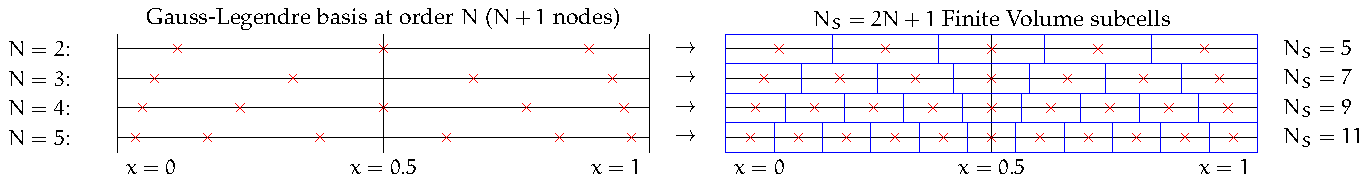
\includegraphics[scale=0.7]{thesis_aderdg_subcell_grid}
  \caption{\label{fig:limiting-subcells}Conversion from \dg{}-dofs to fv-dofs. Image taken from~\cite{dumbser2018conformal}. }
\end{figure}
\todo{Cite source for subcells~\pcref{fig:limiting-subcells}. See guidebook. NOTE THAT IT IS MODIFIED. Also: Fix size, currently font is too small}
For the sake of brevity, we omit technical details.
We refer the interested reader to~\cite{dumbser2016simple}.

%%% Local Variables:
%%% mode: latex
%%% TeX-master: "../main"
%%% End:
